\section{Le Kinect}

\begin{frame}
\tableofcontents[currentsection, hideothersubsections]
\end{frame}

\subsection{Matérielle}
\begin{frame}{Matérielle}
\vbox to 1.0\textheight
{
\begin{block}{Spécifications techniques~\cite{kinect_msdn}\cite{wiki_kinect}}
  \begin{minipage}[t]{0.49\linewidth}
    \begin{itemize}
    \item<1-> \emph{caméra couleur}\only<1->{~:
    \begin{itemize}
    \item 1280x960 à 12Hz,
    \item 640x480 à 30Hz.
    \end{itemize}}
    \item<2-> \emph{étalage de 4 microphones},
    \end{itemize}
  \end{minipage} 
  \begin{minipage}[t]{0.49\linewidth}
    \begin{itemize}
    \item<3-> \emph{capteur de profondeur}\only<3->{~:
    \begin{itemize}
    640x480 à 30Hz.
    \end{itemize}}
    \item<4-> \emph{moteur},
    \item<4-> \emph{accéléromètres}.
    \end{itemize}
  \end{minipage}
\end{block}
  \begin{center}
    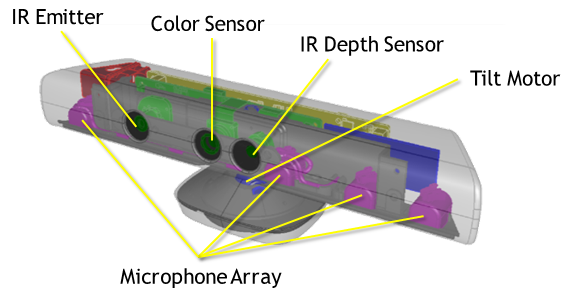
\includegraphics[height=0.4\textheight]{../images/kinect_specs}
  \end{center}
  \vfill
}
\end{frame}

\subsection{Pilotes}
\begin{frame}{Pilotes}

\vbox to 1.0\textheight
{
  \begin{itemize}
  \item sortie du Kinect le 4 Novembre 2010,
  \begin{itemize}
  \item Adafruit offre \$3000 de prime~\cite{adafruit_bounty}.
  
  \only<1>
  {
  \vfill
  \begin{center}
  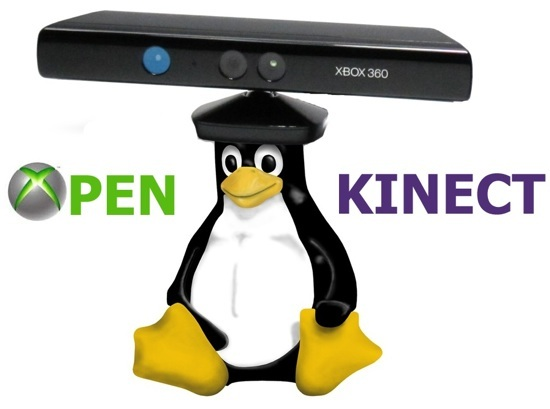
\includegraphics[width=0.65\textheight]{../images/kinect_tux}
  \end{center}
  }
  
  \end{itemize}
    \item<2-> \textbf{Libfreenect} sort le 10 Novembre 2010~\cite{adafruit_winner},
    
    \only<2>
    {
    \vfill
    \begin{center}
    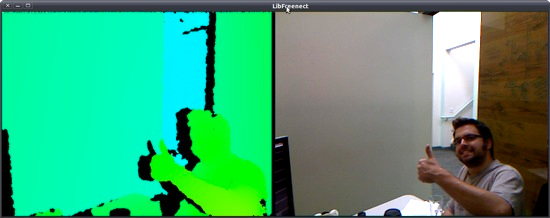
\includegraphics[width=0.9\linewidth]{../images/hector}
    \end{center}
    }
    
    \item<3-> \textbf{CL-NUI} sort le 19 Novembre 2010~\cite{clnui},
    \item<4-> \textbf{Kinect for Windows}~:
    \only<4->
  {
    \begin{itemize}
      \item en bêta le 16 Mai 2011,
      \item version complète le 1 Février 2012,
    \end{itemize}
  }
  \item<5-> \textbf{OpenNI SDK}.
  \end{itemize}
\vfill
}
\end{frame}

\subsection{Middleware}
\begin{frame}{Middleware}

\begin{center}
\only<1>{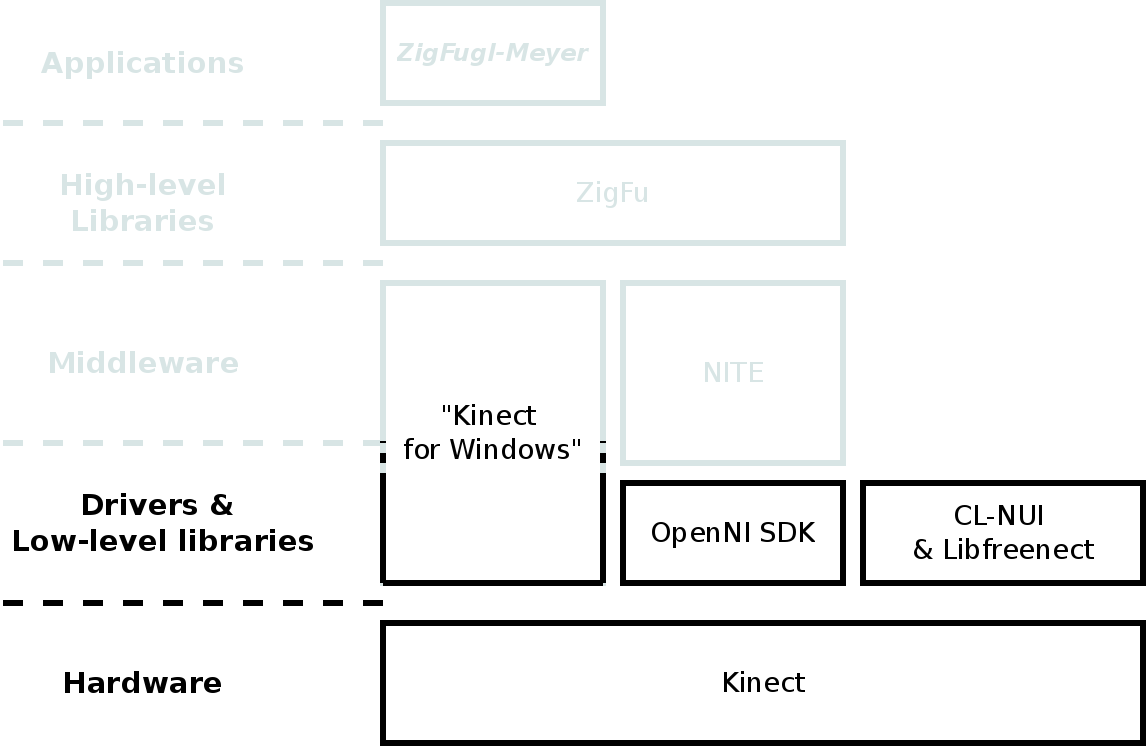
\includegraphics[width=0.9\linewidth]{../images/technology_overview_1}}
\only<2>{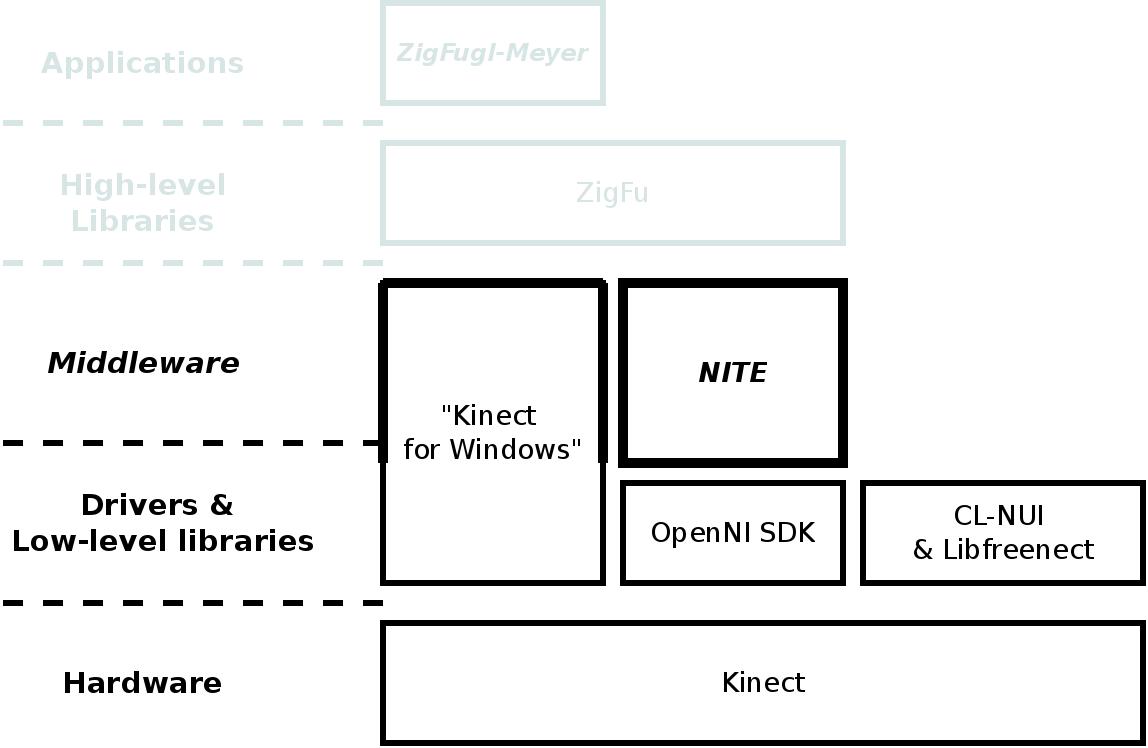
\includegraphics[width=0.9\linewidth]{../images/technology_overview_2}}
\only<3>{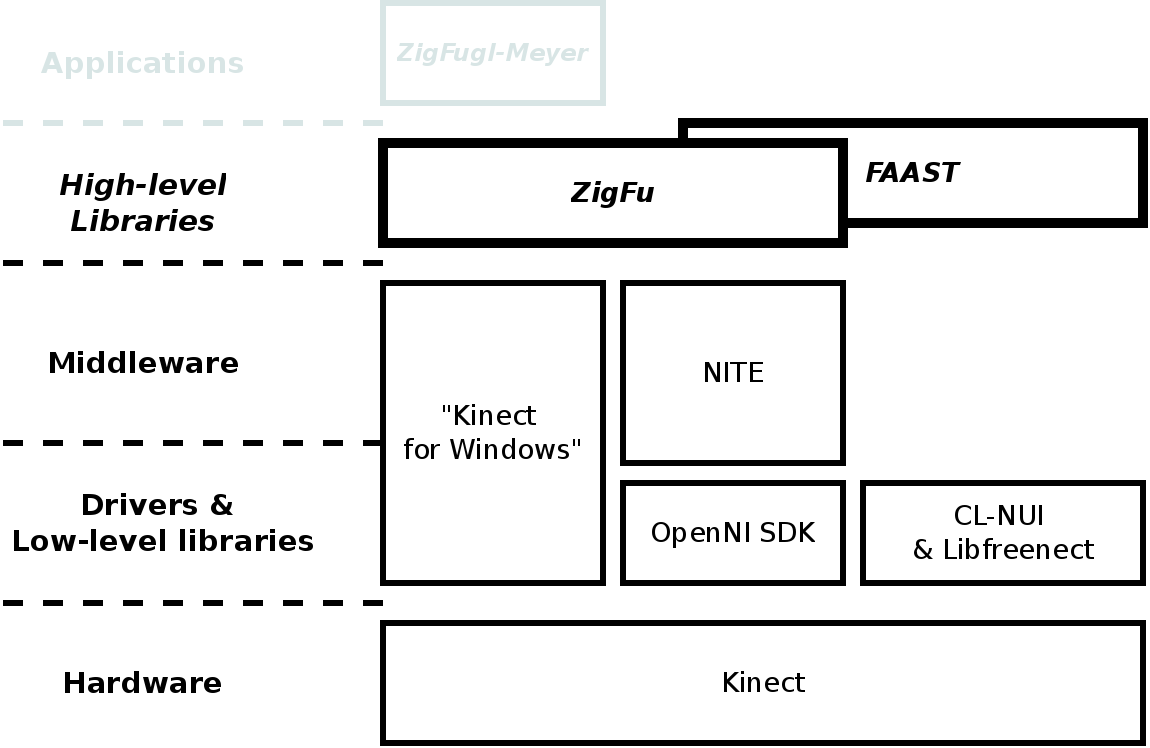
\includegraphics[width=0.9\linewidth]{../images/technology_overview_3}}
\end{center}


\end{frame}

\subsection{Zigfu}
\begin{frame}{Zigfu}
\begin{block}{Features~\cite{zigfu_video}}
  \begin{itemize}
  \item Installation facile, 
  \item Bindings HTML 5, Unity 3D (et Flash bientôt),
  \item Lissage prédictive ($30 \rightarrow 60Hz$), 
  \item Cinématique inverse (simulation physique),
  \item Éléments GUI (boutons, listes, curseurs).
  \end{itemize}
\end{block}
\begin{center}

\includegraphics[width=0.2\linewidth]{../images/zigfu_logo}
\end{center}
\end{frame}

\subsection{Résumé}
\begin{frame}{Résumé}
\begin{center}
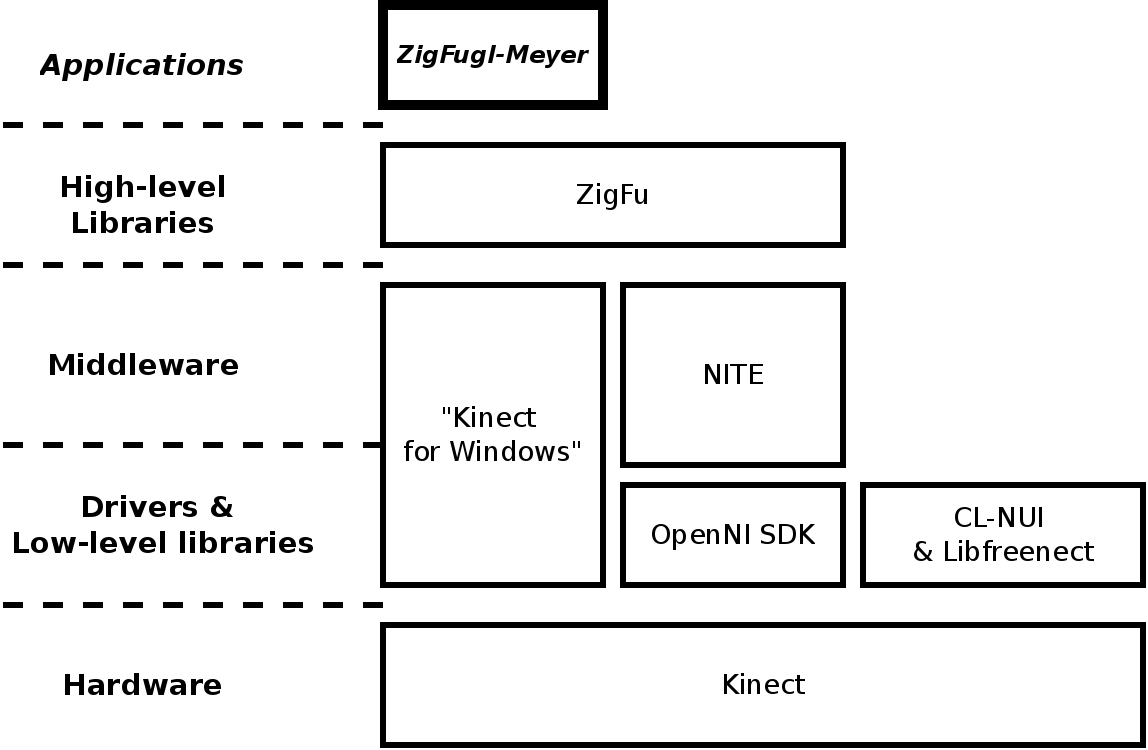
\includegraphics[width=0.9\linewidth]{../images/technology_overview_4}
\end{center}
\end{frame}